\documentclass[10pt, compress]{beamer}

\usetheme{m}

\usepackage{booktabs}
\usepackage[scale=2]{ccicons}
\usepackage{minted}

\usemintedstyle{trac}

\title{Energy efficiency \& optimization for supercomputers}
\subtitle{Parallel Programming course [IN2147]}
\date{May 27, 2015}
\author{Gerasimos Chourdakis}
\institute{Technische Universität München - Supervisor: Prof. Dr. Michael Gerndt}

\begin{document}

\maketitle

\begin{frame}[fragile]{Our path}
    \tableofcontents
\end{frame}

\section{Motivation}

\plain{What is this?}{
    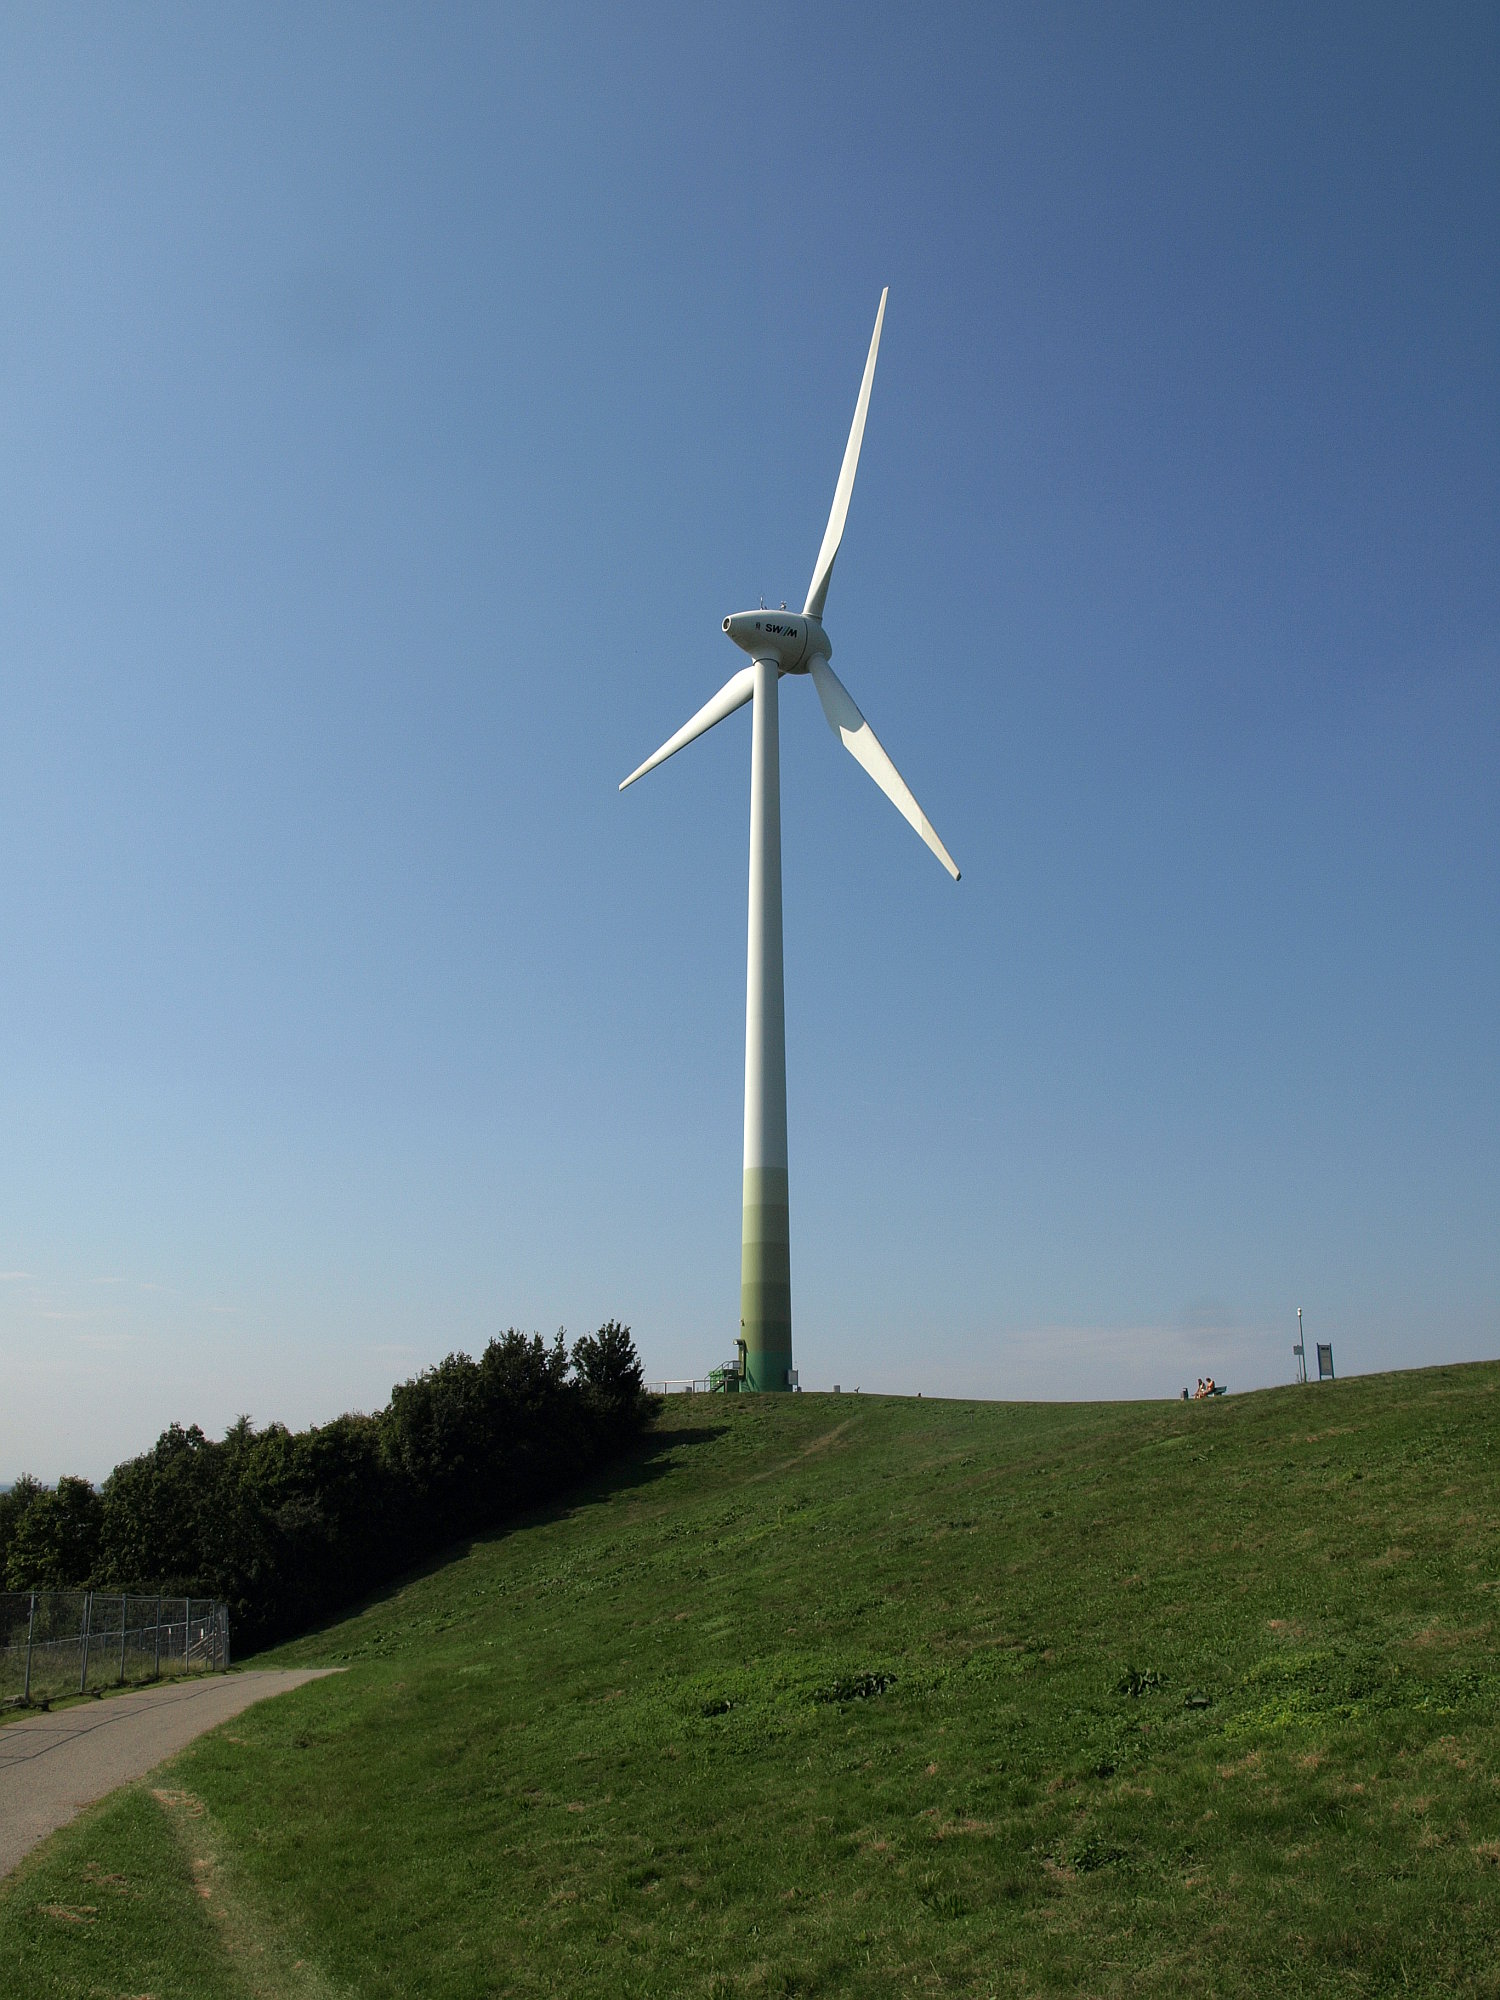
\includegraphics[width=0.5\textwidth]{images/frottmaning.jpg}
}


\begin{frame}[fragile]{Fröttmaning Wind Power Plant}
    Rated power: 1.5 MW
    
    \pause
    
    SuperMUC power consumption: \textasciitilde  3.4 MW
    
    \pause
    
    If this was used to power SuperMUC, it just... \textbf{wouldn't be enough!}
\end{frame}


\begin{frame}[fragile]{The Green500 list}
\textbf{Performance} is important, but it comes at a \textbf{cost}!

The Green500.org list sorts the world's best supercomputers in terms of energy efficiency.

  \begin{table}
    \caption{Part of the Green500 list - November 2014 (rounded numbers)}
    \begin{tabular}{lrrrr}
      \toprule
      Name & \alert{Top500\#} & Green500\# & MFLOPS/W & Power (kW)\\
      \midrule
      Tianhe-2  & 1 & 64 & 1\,902 & 17\,808 \\
      Titan     & 2 & 53 & 2\,143 & 8\,209 \\
      Sequoia   & 3 & 48 & 2\,177 & 7\,890 \\
      K Computer& 4 & 156& 830    & 12\,660 \\
      JUQUEEN   & 8 & 40 & 2\,177 & 2\,301 \\
      SuperMUC  & 14& 152& 846    & 3\,423 \\
      \bottomrule
    \end{tabular}
  \end{table}
\end{frame}


\begin{frame}[fragile]{The Green500 list}
\textbf{Performance} is important, but it comes at a \textbf{cost}!

The Green500.org list sorts the world's best supercomputers in terms of energy efficiency.

  \begin{table}
    \caption{Part of the Green500 list - November 2014 (rounded numbers)}
    \begin{tabular}{lrrrr}
      \toprule
      Name & Top500\# & \alert{Green500\#} & MFLOPS/W & Power (kW)\\
      \midrule
      JUQUEEN   & 8 & 40 & 2\,177 & 2\,301 \\ 
      Sequoia   & 3 & 48 & 2\,177 & 7\,890 \\      
      Titan     & 2 & 53 & 2\,143 & 8\,209 \\
      Tianhe-2  & 1 & 64 & 1\,902 & 17\,808 \\
      SuperMUC  & 14& 152& 846    & 3\,423 \\      
      K Computer& 4 & 156& 830    & 12\,660 \\
      \bottomrule
    \end{tabular}
  \end{table}
\end{frame}



\section{Energy Efficiency}

\subsection{Inside the efficient chips}


\begin{frame}[fragile]{A rough CPU power model}
The \textbf{dominating part} of the power consumption of a CPU is its dynamic power, that is \alert{proportional to its frequency}, and the square of its voltage:

\begin{equation}
 P_{CPU} = P_{dynamic} + P_{short\,circuit} + P_{leakage}
\end{equation}

\begin{equation}
 P_{dynamic} = Capacitance \cdot Voltage^2 \cdot frequency
\end{equation}
\end{frame}


\begin{frame}[fragile]{Energy Management in the CPU}
Modern processors try to save energy in various ways:
\begin{itemize}
\item \alert{Reducing frequency or voltage (DVFS)}
\item Turning unused areas off
\item Reducing capacitance (smaller chips)
\item Recycling energy stored in capacitors, and more.
\end{itemize}

\pause

\textbf{Thinking out-of-the-box:} The ARM architectures are RISC-type, in comparison to
usual x86 CISC architectures. They need less transistors, that roughly means
less power!

\pause

Of course, a supercomputer is not built only with CPUs...
\end{frame}


\subsection{Efficient infrastructure}

\begin{frame}[fragile]{Efficient infrastructure}

Remember: we cannot ignore the energy balance! The electric power that we consume
is transformed to heat.

CPUs have specific operating temperature specifications, so \alert{we need to remove the
produced heat} (cooling).

Also, a supercomputing center does not consume energy only for the supercomputer. A good example: LRZ!
\end{frame}

\begin{frame}[fragile]{Example: Warm-water cooling}
SuperMUC is water-cooled (IBM "Aquasar"). More than this, it is \alert{cooled with warm water}!?!? 

\pause

Do we really need a fridge-cold liquid (cost for chilling)? Typical temperature limit is 85°C
and it is not exceeded even with 60°C "cooling" water.

\pause

Plus: the water at the output contains energy in high temperature, i.e. useful energy!
\alert{All the LRZ buildings can be heated with this "free" energy.}
\end{frame}


\subsection{An energy-efficient future}

\begin{frame}[fragile]{An energy-efficient future}
 We use more and more \textbf{accelerators} in place of more CPU cores. But accelerators are power-greedy!
 
 \pause
 
 What about \textbf{hybrid systems}? For example, ARM CPUs connected with GPUs.
 
 \pause
 
 \textbf{Exa-scale challenges:} could we reliably produce and manage e.g. 20MW of electricity
 just for a supercomputer? Could we also efficiently remove this (condensed) heat?
 
 Keep in mind: electric energy can be cheaper if it is \alert{predictably consumed at a
 constant rate}. This changes our viewpoint: variate the number of nodes to keep the energy constant. (scheduler)
\end{frame}

\section{Energy Optimization}

\subsection{What to optimize}

\begin{frame}[fragile]{What to optimize?}
Remember:

\begin{math}
 P_{dynamic} = Capacitance \cdot Voltage^2 \cdot frequency
\end{math}

So, we could just (easily) decrease the frequency, right? 

Hmm...

\end{frame}

\begin{frame}[fragile]{Energy to Solution}
 We are not actually paying for power, but for energy, i.e. $power \cdot time$.
 
 For which frequency do we get the desired \alert{minimum Energy to Solution}?
 
 Other metrics: Energy Delay Product ($EDP$) or even $ED^nP$. 
\end{frame}

\begin{frame}[fragile]{A model for Energy to Solution}

\begin{equation}
E = \frac{W_0 + (W_1 \cdot f + W_2 \cdot f^2 ) t}{min(t \cdot P_0 \cdot f / f_0 , P_{roof})}
\end{equation}

\begin{equation}
f_{optimal} = \sqrt{\frac{W_0}{w_2 \cdot t}}
\end{equation}

Assumptions:
\begin{enumerate}
\item Certain baseline power $W_0$ is used for the whole (multicore) chip.
\item An active core consumes a dynamic power of $W_1 \cdot f + W_2 \cdot f^2$.
\item At baseline frequency $f_0$ we have a baseline performance $P_0$. A bottleneck
may restrict the performance to $P_{roof}$.
\end{enumerate}
\end{frame}


\subsection{How to get data}
\begin{frame}[fragile]{How to get data?}
We are trying to optimize the "consumed energy", but at which level?

\pause

We could measure the energy consumed at \textbf{hardware level}, by using
the internal CPU event counters. This would give us high \textbf{measurement frequency},
and more \textbf{information} but also an \textbf{overhead} due to in-band measurement and model inaccuracies.

\pause

We could directly measure the energy consumed at \textbf{node or higher level}, by using "smart" power supplies. These give us low frequencies but they can provide useful statistics for \textbf{long-run} applications.
\end{frame}

\subsection{Bob the Builder's tools}

\begin{frame}[fragile]{Bob the Builder's tools}
...or "energy optimization made easy"!

\textbf{Optimize performace first!} For this, we need a profiling tool
to locate the "hot spots" of our code. Already wide-spread tools: gprof, Vampir, Scalasca and other.

\pause

After we optimize performance, what about manipulating \textbf{compiler flags and cpu frequency}?
\end{frame}

\begin{frame}[fragile]{The Periscope Tuning Framework and AutoTune}
TUM, LRZ and other European partners develop the \alert{Periscope Tuning Framework} and the \alert{AutoTune} plugin: \href{http://periscope.in.tum.de/}{periscope.in.tum.de}.

It is an \textbf{online} (no tracing files) analysis and tuning framework for performance and energy, built
to work with Eclipse.

It can help to decide which compiler flags and MPI parameters to use, as well as to find the
optimal CPU frequency for our code.
\end{frame}

\begin{frame}[fragile]{The Periscope Tuning Framework and AutoTune}
\textbf{How does it work?}

Through a graphical user interface, the user sets up the different \textbf{scenarios} to be checked
and provides a test dataset.

The user also selects a \textbf{search algorithm} that compiles and runs the program for the different scenarios in order to find the combination of parameters that gives the optimal execution time or energy metrics.
\end{frame}

\section{Summary}

\begin{frame}[fragile]{Summary}
\begin{itemize}[<+- | alert@+>]
    \item Supercomputers are energy-hungry and there is a good reason in spending a lot of effort 
    to optimize their energy consumption.
    \item CPUs consume less energy at lower frequency, but the energy to solution is what matters. Sometimes, the time to solution is even more important than energy.
    \item The energy consumed by the CPU also produces energy that needs to be removed. Warm-water cooling 
    can decrease the cooling cost and could be paired with other heating processes.
    \item We can optimize based on measurements provided from the CPU or from other equipment, with varying measurement frequency and overhead.
    \item Before we optimize energy consumption, we must have an efficient code. Profiling tools can make our life easier.
    \item The Periscope Tuning Framework is a nice tools that can analyze and fine-tune our code for the specific system that we are using.
\end{itemize}
\end{frame}

\begin{frame}[fragile]{Selected References}
\begin{enumerate}
\item "Tools and methods for measuring and tuning the energy efficiency of HPC systems",
R. Schöne et al., Scientific Programming 22 (2014) 273–283. DOI 10.3233/SPR-140393.
\item "A Case Study of Energy Aware Scheduling on SuperMUC", A. Auweter \& L. Brochard, LRZ, 
30/06/2014. (presentation)
\item "Automatic Tuning of HPC Applications with Periscope", M. Gerndt, M. Firbach and I. Compres, LRZ, 23/04/2015. (presentation)
\end{enumerate}
\end{frame}

\begin{frame}[fragile]{Licensing}
    You can find this presentation on Github:
    \begin{center}\url{https://github.com/MakisH/}\end{center}

  This work is provided with a
  \href{http://creativecommons.org/licenses/by-sa/4.0/}{Creative Commons
  Attribution-ShareAlike 4.0 International License}.

  \begin{center}\ccbysa\end{center}
  
  Picture on slide \#3 belongs to Hochgeladen von Hihiman and is covered by a CC BY-SA 3.0 license. Downloaded from \url{https://de.wikipedia.org/}.
  
  The slides are built with the "m" beamer theme by Matthias Vogelgesang that is provided with a CC BY-SA 4.0 license  and can be found at \url{github.com/matze/mtheme}.
\end{frame}

\plain{}{Questions?}

\end{document}
